\section{簡介}
隨著近年來行動裝置與雲端運算的興起,行動裝置逐漸成為了業界的兵家必爭之地,許多公司都喊出了「行動優先」口號,足見業界對於行動裝置平台之重視,如Google、Facebook、Apple等科技大廠皆紛紛搶入行動裝置平台。由於行動裝置小、鍵盤輸入介面不方便、往往需要在移動時輸入等特性,使得語音輸入在行動裝置上相形重要,因為語音相對於傳統的鍵盤輸入是更自然也更貼近人性的輸入方法。但行動裝置上的語音輸入不比傳統的語音輸入,有許多與傳統語音輸入不同的特性,由於這些特性將導致一些困難的挑戰和更多有趣的性質可供研究,以下將簡介這些特性。

第一個特性為自發性語音 (Spontaneous) 含發音差異 (Pronounciation Variation)、不流暢性 (Disfluency)、語速變化 (Speaking Rate Variation)~\cite{DBLP:conf/interspeech/YehLL13}及背景雜訊 (Background Noise),由於使用者使用行動裝置上的語音輸入時往往是很自發性地 (Spontaneous) 說話,因此這些語速是很不固定的,將隨著使用者的使用情景、當下的情緒等等而改變,另一方面行動輸入通常會在有背景雜音的狀況下輸入,如馬路上、百貨公司中,會附有很多的背景雜音,因此語速變化與背景雜音可以說是行動語音輸入最主要的困難之一。

第二個特性為個人化 (Personalization),這是由於行動裝置通常只屬於某一特定的使用者,因此行動裝置可以搜集大量的個人資訊對使用者進行個人化,使得使用者的語音辨識結果最接近他有可能說出的話。這其中包含了語音模型、語言模型與辭典的個人化~\cite{DBLP:conf/interspeech/WenHLTL13, wen2012personalized, bellegarda2004statistical},語音模型可以調適 (Adaptation) 至接近使用者語音特性的語音模型,語言模型與辭典則可以藉由收集使用者常說與常用的詞
(可以從過去的語音輸入中收集,或是從社群網路如 Facebook、Twitter上收集)進行調適。如此一來即可以將使用者的行動語音輸入個人化成最適合使用者使用的行動語音輸入。

第三個特性為行動裝置上的感測器 (Sensor),這是行動裝置上特有的特性,由於行動裝置上通常帶有全球定位系統 (Global Positioning System, GPS)
,而未來甚至可能帶有個人身體狀況的感測器,如血壓、心跳等,而這些感測器的特徵正好可用來幫助語音辨識,如裝置知道使用者的位置,就可以將當地景點、餐廳在語言模型中的機率增加,如裝置知道使用者血壓、心跳增高,可能代表使用者處於憤怒狀態,此時憤怒的詞彙在語言模型中的機率也可以被適當地增加。因此如果可以擅用這些感測器的結果,將能很好地幫助語音辨識。

本章中的個人化語音系統的應用皆實作於 Google 推出的 Google 眼鏡 (Google Glass) 之上 (如圖~\ref{fig:glass}),Google 眼鏡主體為其右上角之藍色部分,其前面包含了一塊透明的顯示器,Google 眼鏡會將顯示畫面投影到透明的顯示器上讓使用者閱讀,藍色的部分還包含了麥克風、喇叭、相機、觸控板(可偵測多種手勢)等裝置。

\begin{figure}
\centering
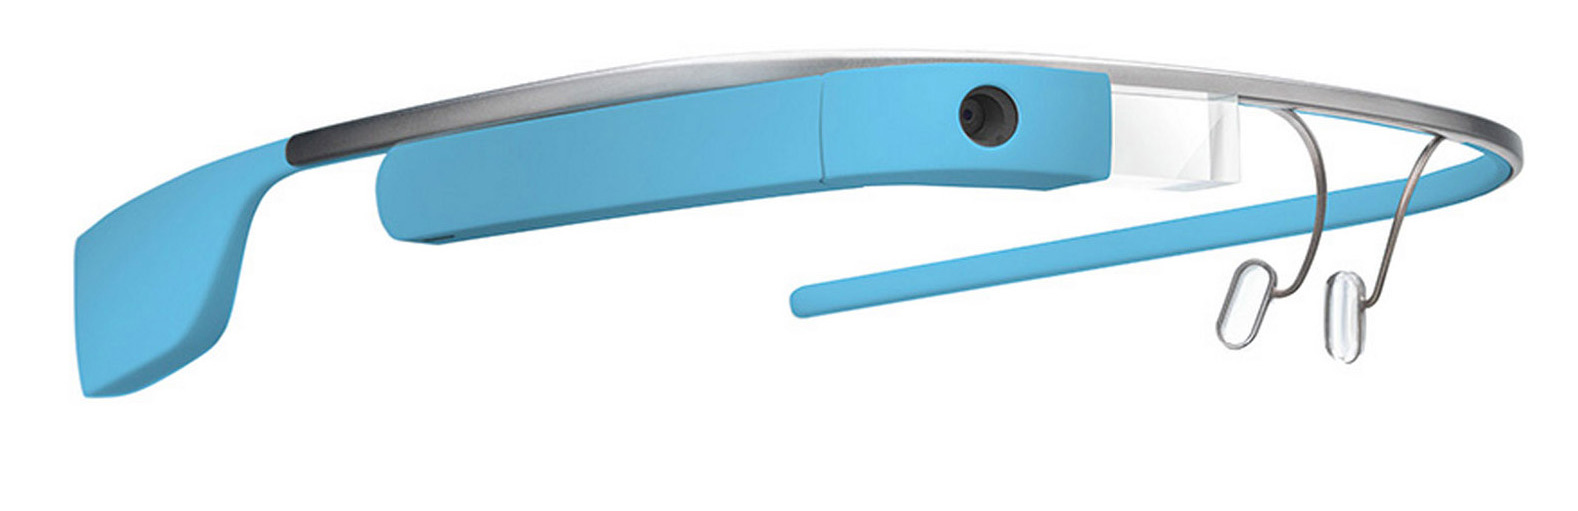
\includegraphics[scale=0.2]{images/glass.jpg}
\caption{Google 眼鏡} \label{fig:glass}
\end{figure}

\section{個人化的語言翻譯系統簡介}

以下將介紹本實驗室開發的個人化語言翻譯系統,其開發動機是由於穿戴型裝置日益流行,如果能讓使用者在旅遊或是與外國人對話的期間,一旦有不會講的話就能直接用自己的母語對裝置說話,並由裝置進行辨識與翻譯後告訴使用者該如何用另一個語言講這段話。

因此我們設計了一套個人化語言翻譯系統,利用智慧型行動裝置如手機、甚至是近年來逐漸受到重視的智慧型穿載裝置,像Google眼鏡等,讓使用者能隨時隨地地進行為自己量身打造的體驗:使用者以自己的母語講出想學的內容,行動裝置會將訊號送至雲端的個人化語音辨識系統,將語音辨識成文字,再將辨識後的文字送至Google提供的翻譯服務將文字翻譯成使用者想學的目標語言,再回傳到行動裝置讓使用者同時看到翻譯後的文字與聽見範例發音,系統示意如圖 ~\ref{fig:chap6_translation_system}

\begin{figure}
\centering
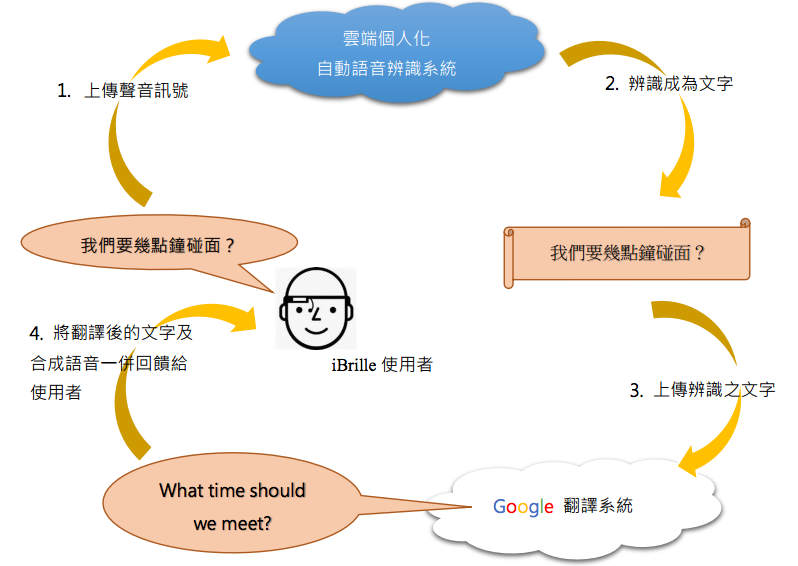
\includegraphics[scale=0.4]{images/chap6_translation_system.png}
\caption{雲端個人化語言翻譯系統架構} \label{fig:chap6_translation_system}
\end{figure}

本系統可分為兩部分:

\subsubsection{個人化自動語音辨識系統 (Personalized Automatic Speech Recognition System)} 
目前使用的雲端辨識系統可分為幾個區塊,包含聲學模型、語言模型、詞典,依序介紹如下:

\begin{itemize}

   \item 聲學模型:

聲學模型架構使用的是三連音(Triphone)隱藏式馬可夫模型(Hidden Markov Model, HMM),每一個馬可夫模態(HMM State)則是由深層類神經網路(Deep Neural Networ)的輸出層中的一個神經元(Neuron)來表示,也就是近年流行的上下文相關深層類神經網路隱藏式馬可夫模型 (Context-dependent Deep Neural Network Hidden Markov Model,
CD-DNN-HMM)。類神經網路端所輸入的語音特徵則是疊加了九個音框長度的梅爾濾波器組特徵(Mel-Filter Bank Features),維度是621維。網路中共有四層隱藏層(Hidden Layer),每一層中有2048個隱藏神經元(Hidden Neuron),輸出層則是有6647個節點。用來訓練聲學模型的語料則是結合了雙語料,其中聲碩麥克風(ASTMIC)做為中文語料以及台灣區英語(English Across Taiwan)當中非母語語者(Non-native Speaker)部分做為英文語料。
兩個語料都是收集自台灣區語者的錄音,並且都是多語者(Multi-speaker)語料,且性別各半均衡。

   \item 語言模型:

語言模型採用傳統的N連詞(N-gram)模型,並且為三連詞模型。訓練語料包含了Yahoo! 新聞(Yahoo! News)、 Gigaword、公視新聞 (PTV),並且在訓練完成後,與以聲碩麥克風與台灣區英語的訓練集語料訓練的語言模型作內插調適。

   \item 詞典:

此系統詞典中文部分包含所有常見中文單字,以及經由PAT-Tree所產生的
字詞。英文部分,則是包含卡內基美儂大學所公開之英文辭典當中,詞頻較高者。所有字詞的發音皆是音素(Phoneme)序列,包含中英雙語的所有音素。

\end{itemize}

\subsubsection{翻譯系統}

經辨識所得之文字,將送至 Google 的雲端翻譯系統,並由 Google 翻譯將其翻譯為使用者想學的目標語言,再將翻譯後的文字與合成發音一併傳回    Google 眼鏡上,將使用者想翻譯的語言呈現於屏幕上,並同步撥放發音以助翻譯。此一部分由於本實驗室尚未有完善的翻譯系統,不過一旦未來研發出辨識系統後,即可將 Google 翻譯系統替換為本實驗室自行開發之翻譯系統。

\section{個人化的語音文件檢索系統簡介}
以下將介紹本實驗室自行開發的個人化行動語音文件檢索系統,其開發動機為使用者在行動時也往往有搜尋資訊的需求,而在移動時使用鍵盤輸入對於使用者又極度地不方便,因此我們就決定開發了這套基於 Google 眼鏡的語音文件檢索系統,讓使用者能夠隨時隨地取得自己想要的資訊,使用情境如下:使用者對 Google 眼鏡輸入語音查詢詞,然後 Google 眼鏡再將訊號上傳到個人化語音辨識系統,辨識為文字後,系統再將文字的語音查詢詞上傳至
~\ref{sec:chap4_semantic_retrieval} 中提到的監督式語意文件檢索系統。檢索系統會再將檢索後的內容傳回給使用者,並呈現於 Google 眼鏡上供使用者閱讀。

本系統可分為兩部分:

\subsubsection{個人化自動語音辨識系統}

此部分同上一節個人化的語言翻譯系統中的個人化語音辨識系統。

\subsubsection{監督式語意檢索系統}

此處使用之系統同~\ref{sec:chap4_semantic_retrieval},使用的語料為2001年間從電台廣播中錄下的4小時新聞,並手動切成5034篇語音文件,每篇語音文件大約包含了1至3句的語句。用來辨識的語言模型是用1999年間收集的新聞文章 (包含4000萬個詞彙) 訓練而成,辭典中包含了62000個詞彙,聲學模型是用2000年間收集的8小時廣播新聞訓練而成的音節內(Intra-syllable)
右方資訊相依(Right-context-dependent) 聲韻母模型 (Initial-Final models)。辨識後的唯一最佳序列的字元正確率為 (Character Accuracy) 為75.27\%。
\section{系統展示}
此節將展示本系統之部分截圖與使用示例。

\subsection{個人化的語音翻譯系統展示}
本實驗室開發的個人化語音翻譯系統的名稱取為iBrille,取Brille在德語中為眼鏡,在西班牙語及法語中有閃耀的意思。圖 ~\ref{fig:ibrille_enter} 中為 iBrille 系統的首頁,一進入系統後會顯示「觀迎來到 iBrille 教學系統」,圖 ~\ref{fig:ibrille_example} 中則為使用者對 iBrille 講出一段欲翻譯的話後,由個人化的語音翻譯系統辨識、並翻譯後顯示的畫面。
\begin{figure}
\centering
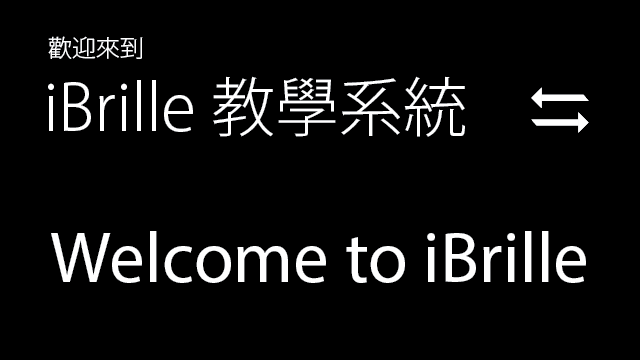
\includegraphics[scale=0.3]{images/glass/ibrille_enter.png}
\caption{iBrille 首頁} \label{fig:ibrille_enter}
\centering

\includegraphics[scale=0.3]{images/glass/ibrille_example.png}
\caption{iBrille 使用示範} \label{fig:ibrille_example}
\end{figure}

\subsection{個人化的語音文件檢索系統展示}
本實驗室開發的個人化語音文件檢索系統的名稱取為「新聞隨手查」,希望能讓使用者無論在隨時隨地都能很方便迅速地吸收到感興趣的資訊。圖 ~\ref{fig:news_enter} 為新聞隨手查的首頁,而圖 ~\ref{fig:news_example} 則為使用者說出「颱風」這個查詢詞後顯示的畫面。
\begin{figure}
\centering
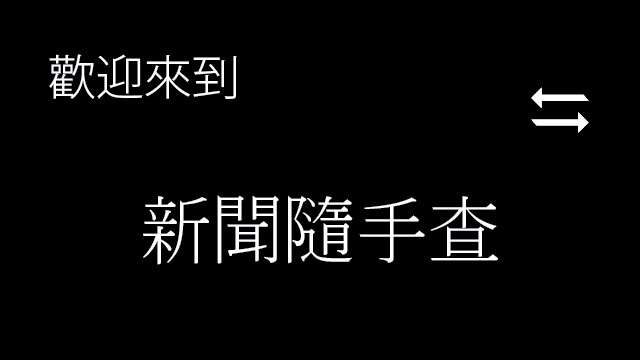
\includegraphics[scale=0.3]{images/glass/news_enter.png}
\caption{新聞隨手查首頁} \label{fig:news_enter}
\centering
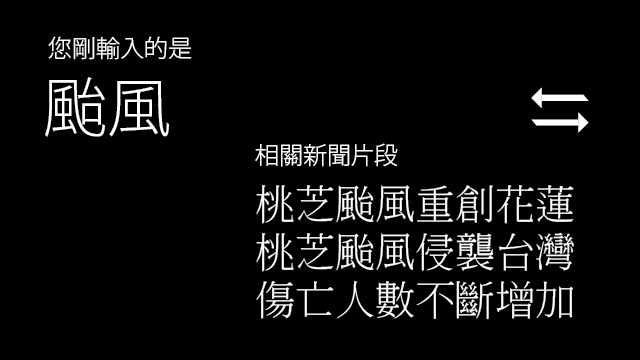
\includegraphics[scale=0.3]{images/glass/news_example.png}
\caption{新聞隨手查使用示範} \label{fig:news_example}
\end{figure}

\section{本章總結}
行動裝置在這幾年內漸形重要,因此也使得在行動裝置上的語言輸入漸受重視,本章中利用了 Google 眼鏡實作了個人化的語音翻譯系統與個人化的語音文件檢索系統,將個人化的語音辨識系統與行動裝置上的應用程序結合起來,成為對使用者更為方便的應用程序。
